\chapter{बोल्ट्ज़मान गुणक}\label{ch:b2:boltzmann-factor}

किसी पहाड़ पर चढ़िए और हवा पतली होती जाती है: तीन हज़ार मीटर पर
दाब गिरकर \qty{0.7}{bar} रह जाता है, और एवरेस्ट की चोटी पर समुद्र-तल के
मान का एक-तिहाई। ऊपर से वायुमंडल को कुछ नहीं बाँधता; उसे गुरुत्व थामे रखता
है और तापीय क्षोभ फैलाता है, और दोनों के बीच का समझौता कोई चरघातांकी है, $n \propto
\eu^{-mgz/k_BT}$ --- किसी अणु की स्थितिज ऊर्जा का
$k_BT$ से अनुपात तय करता है कि वह ऊपर कितनी दुर्लभ है। वही चरघातांकी शासित करती है
किसी उत्तेजित स्तर में परमाणुओं का अंश, इतने तेज़ अणुओं की संख्या
कि वे किसी ग्रह से भाग सकें, किसी अनुचुंबक का चुंबकन, वे जनसंख्याएँ
जिन्हें किसी \omterm{def:b2:laser:cavity}{लेज़र} को उलटना पड़ता है, और वे क्वांटा जिन्हें प्लांक का नियम
गिनता है: यही है \emph{बोल्ट्ज़मान गुणक}, सांख्यिकीय भौतिकी का सबसे उपयोगी
अकेला सूत्र। यह अध्याय उसे वायुमंडल से प्रेरित करता है,
उसे व्यापक रूप में कहता है, और उससे, योगों तथा गाउसी समाकलों के सिवा कुछ न लेकर,
द्विस्तरीय निकाय और उसकी ऊष्मा-धारिता, ऊर्जा का समविभाजन,
आणविक चालों का वितरण, और अनुचुंबकत्व का क्यूरी नियम खींचता है --- और रास्ते में,
किसी क्वांटम दोलक की माध्य ऊर्जा, जो प्लांक का सूत्र है।

\begin{omfigure}

\includegraphics[width=0.58\linewidth]{images/book4/ai/b4-29-sky-gradient-summit.png}

{\small किसी शिखर से, निचले वायुमंडल का धुँधलका और ऊपर का गहरा
नीला: हवा का घनत्व हर \qty{8}{km} पर $\eu$ गुने से गिरता है
--- पृथ्वी के गुरुत्व में किसी अणु की स्थितिज ऊर्जा का
बोल्ट्ज़मान गुणक।}
\end{omfigure}

\section{समतापी वायुमंडल}

\begin{proposition}[वायुदाबमापी नियम]\label{prop:b2:boltzmann-factor:barometric}
परिपूर्ण गैस (आणविक द्रव्यमान $m$) के किसी वायुमंडल में, एकसमान
ताप $T$ पर एकसमान गुरुत्व $g$ में, दाब और संख्या-घनत्व
ऊँचाई के साथ चरघातांकी रूप से गिरते हैं:
\[
P(z) = P_0\,\eu^{-z/H}, \qquad n(z) = n_0\,\eu^{-mgz/k_BT}, \qquad
H = \frac{k_BT}{mg} ,
\]
जिसमें \emph{मापक ऊँचाई}\index{मापक ऊँचाई} $H \approx \qty{8.4}{km}$
\qty{288}{K} पर हवा के लिए। चरघातांक किसी अणु की स्थितिज
ऊर्जा $mgz$ का तापीय ऊर्जा $k_BT$ से अनुपात है।
\end{proposition}

\begin{proof}
द्रवस्थैतिकी, $\dd P/\dd z = -\rho g = -nmg$, और परिपूर्ण-गैस नियम $P
= nk_BT$: $\dd P/\dd z = -(mg/k_BT)P$, कोई चरघातांकी। असली
वायुमंडल ऊँचाई के साथ ठंडा होता है (सबसे निचले दस किलोमीटर में लगभग
\qty{6.5}{K/km}), जो गिरावट को कुछ तेज़ कर देता है; समतापी
मॉडल $20\%$ तक अच्छा है।
\end{proof}

\begin{omfigure}
\begin{tikzpicture}
  \begin{axis}[omaxis, width=8.2cm, height=4.8cm, xmin=0, xmax=32, ymin=0, ymax=1.1,
    xlabel={$z$ (\unit{km})}, ylabel={$P/P_0$}, xtick={8.4,16.8,25.2}, xticklabels={$H$,$2H$,$3H$}, ytick={0.37,1}, yticklabels={$1/\eu$,$1$}, clip=false,
    legend style={font=\scriptsize, at={(0.97,0.45)}, anchor=north east, draw=none, fill=none}]
    \addplot[omDef, thick, domain=0:32, samples=80] {exp(-x/8.4)};
    \addlegendentry{हवा, \qty{288}{K}}
    \addplot[omExo, thick, dashed, domain=0:32, samples=80] {exp(-x/60)};
    \addlegendentry{केवल हीलियम, $H = \qty{60}{km}$}
    \draw[dashed, gray] (axis cs:8.4,0) -- (axis cs:8.4,0.37) -- (axis cs:0,0.37);
  \end{axis}
\end{tikzpicture}

{\small समतापी वायुमंडल: दाब और घनत्व $1/\eu$ गुने से गिरते हैं हर
\omterm{prop:b2:boltzmann-factor:barometric}{मापक ऊँचाई} $H = k_BT/mg$ पर; किसी हलकी गैस का $H$ बड़ा होता
--- पर \qty{100}{km} से नीचे विक्षोभ हवा को मिलाए रखता है, और सभी
गैसें माध्य $H$ बाँटती हैं।}
\end{omfigure}

\section{बोल्ट्ज़मान गुणक}

\begin{theorem}[बोल्ट्ज़मान गुणक]\label{thm:b2:boltzmann-factor:factor}
ताप $T$ पर किसी तापस्थापी के साथ तापीय साम्य में कोई निकाय
ऊर्जा $E$ की किसी दी हुई सूक्ष्मदर्शी अवस्था में इस
प्रायिकता के अनुपात में पाया जाता है
\[
\eu^{-E/k_BT} .
\]
अतः, ऊर्जाओं $E_i$ की विविक्त अवस्थाओं के किसी समुच्चय के लिए,
\[
p_i = \frac{\eu^{-E_i/k_BT}}{Z}, \qquad Z = \sum_i\eu^{-E_i/k_BT} ,
\]
जिसमें योग $Z$ (वह \emph{विभाजन फलन}\index{विभाजन फलन})
प्रायिकताओं को प्रसामान्यित करता है; दो अवस्थाएँ (या बराबर
अपभ्रष्टता के दो स्तर) अनुपात $N_2/N_1 = \eu^{-(E_2 - E_1)/k_BT}$ में भरी होती हैं;
और किसी संतत चर (कोई स्थिति, कोई वेग) के लिए प्रायिकता
घनत्व उस चर में $\eu^{-E/k_BT}$ के अनुपात में है।
\qty{300}{K} पर, $k_BT = \qty{4.1e-21}{J} = \qty{0.026}{eV}$: जो कुछ इससे
कहीं अधिक महँगा हो वह दुर्लभ है, और जो कहीं कम हो वह
मुक्त रूप से उत्तेजित।
\end{theorem}

\begin{proof}
वायुदाबमापी नियम स्थितिज ऊर्जा $mgz$ के लिए वही गुणक है; हम
उसकी व्यापकता मान लेते हैं, पर तर्क यहाँ है (वर्ष 3 के खंड में कठोर बनाया गया)।
तापस्थापी $R$ बड़ा है; जब हमारा छोटा निकाय
ऊर्जा $E$ की किसी अवस्था में हो, तो तापस्थापी की ऊर्जा $E_{\text{कुल}} -
E$ होती है, और वह $\Omega_R(E_{\text{कुल}} - E)$ सूक्ष्मदर्शी अवस्थाओं में हो सकता है, सभी
समान रूप से प्रायिक (किसी विलगित पूर्ण के लिए मूलभूत अभिगृहीत)। अतः
$p(E) \propto \Omega_R(E_{\text{कुल}} - E)$। एंट्रॉपी की बोल्ट्ज़मान परिभाषा
$S_R = k_B\ln\Omega_R$ के साथ, और तापस्थापी के लिए $1/T = \dd S_R/\dd E_R$,
$\ln\Omega_R(E_{\text{कुल}} - E) \approx \ln\Omega_R(E_{\text{कुल}})
- E/k_BT$ चूँकि $E \ll E_{\text{कुल}}$; अब चरघातांकित कीजिए।
\end{proof}

\begin{example}[परमाण्विक स्तरों की जनसंख्याएँ]\label{ex:b2:boltzmann-factor:levels}
हाइड्रोजन का पहला उत्तेजित स्तर मूल अवस्था से \qty{10.2}{eV} ऊपर पड़ता है:
\qty{300}{K} पर, $\eu^{-395}$ --- ब्रह्मांड भर में एक भी परमाणु नहीं; और
\qty{6000}{K} पर, सूर्य की सतह, $\eu^{-19.7} \approx 3 \times 10^{-9}$ (गुना
$4$ की अपभ्रष्टता): पर्याप्त, सूर्य के विशाल गैस-स्तंभ में,
बामर अवशोषण रेखाओं के लिए, जो \qty{10000}{K} के पास के तारों में सबसे तीखी हैं।
किसी \qty{2500}{K} की लौ में सोडियम की D रेखा (\qty{2.1}{eV}): परमाणुओं का $\eu^{-9.8} = 6
\times 10^{-5}$ अंश उत्तेजित होता है, जो चुटकी भर नमक की पीली लौ
देता है। और \cref{ch:b2:laser} का \omterm{def:b2:laser:cavity}{लेज़र} माध्यम: गुणक
कहता है कि साम्य पर उसका ऊपरी स्तर खाली है, और पंप को उससे लड़ना ही पड़ता है।
\end{example}

\section{विविक्त स्तर: द्विस्तरीय निकाय और दोलक}

\begin{proposition}[विभाजन फलन से माध्य ऊर्जा]\label{prop:b2:boltzmann-factor:meanE}
$\beta = 1/k_BT$ के साथ,
\[
\langle E\rangle = \sum_ip_iE_i = -\frac{\partial\ln Z}{\partial\beta}, \qquad
C = \frac{\dd\langle E\rangle}{\dd T} .
\]
\end{proposition}

\begin{proof}
$\partial_\beta Z = -\sum E_i\eu^{-\beta E_i}$, अब $Z$ से भाग दीजिए।
\end{proof}

\begin{proposition}[द्विस्तरीय निकाय]\label{prop:b2:boltzmann-factor:twolevel}
$N$ स्वतंत्र निकाय जिनके दो स्तर $0$ और $\varepsilon$ हों (किसी क्षेत्र में
प्रचक्रण, एक उत्तेजित स्तर वाले परमाणु, दो स्थितियों वाले दोष):
\[
\frac{N_2}{N} = \frac{1}{\eu^{\varepsilon/k_BT} + 1}, \qquad
\langle E\rangle = \frac{N\varepsilon}{\eu^{\varepsilon/k_BT} + 1}, \qquad
C = Nk_B\,\frac{x^2\eu^x}{(\eu^x + 1)^2}, \quad x = \frac{\varepsilon}{k_BT} .
\]
ऊपरी स्तर नीचे ताप पर खाली है और ऊँचे ताप पर अधिक से अधिक
आधा भरा (साम्य पर कभी उलटा नहीं); ऊष्मा-धारिता
दोनों सिरों पर लुप्त होती है और $0.44\,Nk_B$ पर शिखर पाती है $k_BT = 0.42
\varepsilon$ के पास --- वह \emph{शॉट्की विसंगति}\index{शॉट्की विसंगति},
स्पेक्ट्रम में किसी अंतराल की पहचान।
\end{proposition}

\begin{proof}
$Z = 1 + \eu^{-x}$; $p_2 = \eu^{-x}/(1 + \eu^{-x})$; अब $\langle
E\rangle$ का $T$ के सापेक्ष अवकलन कीजिए।
\end{proof}

\begin{omfigure}
\begin{tikzpicture}
  \begin{axis}[omaxis, width=6.4cm, height=4.4cm, xmin=0, xmax=3.2, ymin=0, ymax=1.1,
    xlabel={$k_BT/\varepsilon$}, ylabel={जनसंख्याएँ}, xtick={1,2,3}, ytick={0.5,1}, clip=false]
    \addplot[omDef, thick, domain=0.02:3.2, samples=100] {1/(exp(1/x)+1)};
    \addplot[omExo, thick, domain=0.02:3.2, samples=100] {exp(1/x)/(exp(1/x)+1)};
    \node[font=\scriptsize, omExo] at (axis cs:1.4,0.85) {$N_1/N$};
    \node[font=\scriptsize, omDef] at (axis cs:1.4,0.2) {$N_2/N$};
  \end{axis}
  \begin{axis}[omaxis, width=6.4cm, height=4.4cm, xmin=0, xmax=3.2, ymin=0, ymax=0.55, xshift=6.6cm,
    xlabel={$k_BT/\varepsilon$}, ylabel={$C/Nk_B$}, xtick={1,2,3}, ytick={0.44}, clip=false]
    \addplot[omThm, thick, domain=0.08:3.2, samples=120] {(1/x)^2*exp(1/x)/(exp(1/x)+1)^2};
    \draw[dashed, gray] (axis cs:0.42,0) -- (axis cs:0.42,0.44);
    \node[font=\scriptsize, below] at (axis cs:0.42,0) {$0.42$};
  \end{axis}
\end{tikzpicture}

{\small द्विस्तरीय निकाय: ताप के सामने जनसंख्याएँ (ऊपरी
स्तर आधे की ओर भरता है, उससे आगे कभी नहीं) और शॉट्की ऊष्मा-धारिता,
कोई उभार वहाँ जहाँ $k_BT$ अंतराल से मेल खाए।}
\end{omfigure}

\begin{proposition}[क्वांटम दोलक और प्लांक का सूत्र]\label{prop:b2:boltzmann-factor:oscillator}
आवृत्ति $\nu$ के किसी हरात्मक दोलक के स्तर $E_n = nh\nu$ हैं (और एक
अचर); ताप $T$ पर,
\[
Z = \frac{1}{1 - \eu^{-h\nu/k_BT}}, \qquad
\langle E\rangle = \frac{h\nu}{\eu^{h\nu/k_BT} - 1}
\ \longrightarrow\
\begin{cases} k_BT & (h\nu \ll k_BT), \\ h\nu\,\eu^{-h\nu/k_BT} & (h\nu \gg k_BT). \end{cases}
\]
यह \omterm{thm:b2:dipole-radiation:field}{विकिरण क्षेत्र} की किसी मोड की वही माध्य ऊर्जा है जिसे प्लांक का
नियम (\cref{ch:b2:thermal-radiation}) मोडों की संख्या से गुणा करता है,
और किसी ठोस में किसी कंपन की माध्य ऊर्जा: ऊँचे ताप पर
चिरसम्मत $k_BT$, और नीचे ताप पर कोई जमी हुई मोड।
\end{proposition}

\begin{proof}
गुणोत्तर श्रेणी, फिर $-\partial_\beta\ln Z$।
\end{proof}

\begin{example}[ठोसों की ऊष्मा-धारिता]\label{ex:b2:boltzmann-factor:einstein}
किसी ठोस के हर परमाणु को समान आवृत्ति $\nu$ के तीन दोलक मानिए
(आइंस्टाइन, 1907): $C = 3Nk_B\,x^2\eu^x/(\eu^x - 1)^2$ जिसमें $x =
h\nu/k_BT$। $\theta_{\text{E}} = h\nu/k_B$ के ऊपर, $C \to 3Nk_B = 3R$ प्रति मोल
--- ड्यूलों और प्टी का नियम (\qty{25}{J/mol/K}), जिसे सीसा,
ताँबा, लोहा कमरे के ताप पर मानते हैं; उससे कहीं नीचे, $C$ ढह जाता है। हीरे
($\theta_{\text{E}} \approx \qty{1300}{K}$) के पास \qty{300}{K} पर केवल \qty{6}{J/mol/K}
है, जिसे चिरसम्मत भौतिकी समझा नहीं सकी, और हर ठोस की
ऊष्मा-धारिता नीचे ताप पर लुप्त हो जाती है --- विकिरण के बाहर क्वांटम की पहली सफलता।
\end{example}

\section{समविभाजन और मैक्सवेल का वितरण}

\begin{theorem}[ऊर्जा का समविभाजन]\label{thm:b2:boltzmann-factor:equipartition}
हर वह चर $q$ जो ऊर्जा में द्विघाती रूप से घुसे, $E = aq^2 +
\dots$, और सभी वास्तविक मानों पर फैले, साम्य पर माध्य ऊर्जा में
$\tfrac12k_BT$ का योगदान करता है:
\[
\langle aq^2\rangle = \tfrac12k_BT .
\]
किसी एक-परमाणुक गैस (तीन स्थानांतरण) का $U = \tfrac32Nk_BT$ और प्रति मोल $C_V =
\tfrac32R$ है; कोई द्वि-परमाणुक गैस दो घूर्णन जोड़ती है, $C_V = \tfrac52R$,
और उसका कंपन (दो द्विघाती पद, पर कमरे के ताप पर $h\nu \gg
k_BT$ के साथ क्वांटित) कुछ हज़ार केल्विन तक जमा रहता है।
\end{theorem}

\begin{proof}
$q$ में प्रायिकता घनत्व $\propto\eu^{-aq^2/k_BT}$ है, कोई गाउसी:
\[
\langle aq^2\rangle = \frac{\int aq^2\,\eu^{-aq^2/k_BT}\,\dd q}{\int\eu^{-aq^2/k_BT}\,\dd q} = \tfrac12k_BT
\]
($\int\eu^{-\lambda q^2}\dd q = \sqrt{\pi/\lambda}$ का $\lambda$ के सापेक्ष
अवकलन कीजिए)। परिणाम को संतत सातत्य चाहिए: जब
स्तरों की दूरी $k_BT$ से अधिक हो तो गुणक चर को जमा देता है,
जैसा ऊपर दोलक के लिए।
\end{proof}

\begin{theorem}[मैक्सवेल का चालों का वितरण]\label{thm:b2:boltzmann-factor:maxwell}
$T$ पर किसी गैस में, वेग-घटक प्रसरण $k_BT/m$ के स्वतंत्र गाउसी हैं,
और चाल $v = |\vect v|$ का प्रायिकता
घनत्व है
\[
f(v) = 4\pi\Big(\frac{m}{2\pi k_BT}\Big)^{3/2}v^2\,\eu^{-mv^2/2k_BT} ,
\]
जिसमें सर्वाधिक संभाव्य, माध्य तथा वर्ग-माध्य-मूल चालें
\[
v_{\text{सं}} = \sqrt{\frac{2k_BT}{m}}, \qquad
\langle v\rangle = \sqrt{\frac{8k_BT}{\pi m}}, \qquad
v_{\text{वमम}} = \sqrt{\frac{3k_BT}{m}} ,
\]
अनुपातों $1 : 1.13 : 1.22$ में हैं। \qty{300}{K} पर नाइट्रोजन के लिए: \qty{422}{},
\qty{476}{}, \qty{517}{m/s}; हाइड्रोजन के लिए, $3.7$ गुना अधिक; और
वितरण की पूँछ, $\propto\eu^{-mv^2/2k_BT}$, वही है जो
सबसे तेज़ अणुओं को वाष्पित होने, अभिक्रिया करने, या कोई ग्रह छोड़ने देती है।
\end{theorem}

\begin{proof}
गतिज ऊर्जा $\tfrac12m(v_x^2 + v_y^2 + v_z^2)$ कोई गुणक
$\eu^{-mv_x^2/2k_BT}\eu^{-mv_y^2/2k_BT}\eu^{-mv_z^2/2k_BT}$ देती है: तीन स्वतंत्र
गाउसी, हर एक $\sqrt{m/2\pi k_BT}$ से प्रसामान्यित। चाल-वितरण
त्रिज्या $v$ और आयतन $4\pi v^2\dd v$ के कोश के सभी वेग बटोरता
है। फिर $v_{\text{सं}}$ को $\dd f/\dd v = 0$ से, और
आघूर्णों को $\int_0^\infty v^3\eu^{-av^2}\dd v = 1/2a^2$, $\int_0^\infty
v^4\eu^{-av^2}\dd v = \tfrac38\sqrt{\pi/a^5}$ से; $v_{\text{वमम}}$ समविभाजन से भी
निकलता है, $\tfrac12m\langle v^2\rangle = \tfrac32k_BT$।
\end{proof}

\begin{omfigure}
\begin{tikzpicture}
  \begin{axis}[omaxis, width=9cm, height=5cm, xmin=0, xmax=1750, ymin=0, ymax=0.0028,
    xlabel={$v$ (\unit{m/s})}, ylabel={$f(v)$}, xtick={400,800,1200}, ytick=\empty, clip=false,
    legend style={font=\scriptsize, at={(0.97,0.95)}, anchor=north east, draw=none, fill=none}]
    \addplot[omDef, thick, domain=0:1600, samples=160] {4*pi*(28*1.66e-27/(2*pi*1.38e-23*100))^1.5*x^2*exp(-28*1.66e-27*x^2/(2*1.38e-23*100))};
    \addlegendentry{N$_2$, \qty{100}{K}}
    \addplot[omThm, thick, domain=0:1600, samples=160] {4*pi*(28*1.66e-27/(2*pi*1.38e-23*300))^1.5*x^2*exp(-28*1.66e-27*x^2/(2*1.38e-23*300))};
    \addlegendentry{N$_2$, \qty{300}{K}}
    \addplot[omExo, thick, domain=0:1600, samples=160] {4*pi*(28*1.66e-27/(2*pi*1.38e-23*1000))^1.5*x^2*exp(-28*1.66e-27*x^2/(2*1.38e-23*1000))};
    \addlegendentry{N$_2$, \qty{1000}{K}}
  \end{axis}
\end{tikzpicture}

{\small तीन तापों पर नाइट्रोजन के लिए मैक्सवेल का चाल-वितरण:
शिखर $\sqrt T$ की तरह खिसकता है, वक्र चौड़ा होता है, और
ऊँची-चाल वाली पूँछ सबसे तेज़ बढ़ती है --- वही पूँछ जो पलायन
तथा अभिक्रिया-दर तय करती है।}
\end{omfigure}

\begin{example}[ग्रह कौन छोड़ता है]\label{ex:b2:boltzmann-factor:escape}
पृथ्वी की पलायन चाल \qty{11.2}{km/s} है। बहिर्मंडल में, लगभग
\qty{1000}{K} पर, हीलियम का $v_{\text{सं}} = \qty{2.0}{km/s}$ है: पलायन चाल से ऊपर
परमाणुओं का अंश कोटि $\eu^{-(11.2/2.0)^2} = \eu^{-31}
\approx 10^{-13}$ का है --- छोटा, पर अरबों वर्षों तक हर टक्कर पर नया
होता रहा: हीलियम रिसकर चला जाता है, और हवा में उसकी बहुतायत केवल
\qty{5}{ppm} है, रेडियोऐक्टिव क्षय से उसके लगातार उत्पादन के बावजूद।
नाइट्रोजन के लिए चरघातांक सात गुना बड़ा है, $\eu^{-220}$: नाइट्रोजन ठहरता है।
चंद्रमा पर ($v_{\text{पल}} = \qty{2.4}{km/s}$) \qty{400}{K} पर नाइट्रोजन तक
($v_{\text{सं}} = \qty{490}{m/s}$) का प्रति टक्कर-काल $\eu^{-24}$ है:
सौर मंडल की आयु भर में, कोई वायुमंडल नहीं बचता।
\end{example}

\section{अनुचुंबकत्व और क्यूरी नियम}

\begin{proposition}[प्रचक्रण-1/2 अनुचुंबक]\label{prop:b2:boltzmann-factor:curie}
$N$ स्वतंत्र चुंबकीय आघूर्ण जो केवल क्षेत्र $B$ के अनुदिश या उसके
विरुद्ध संकेत कर सकें, ऊर्जाओं $\mp\mu B$ के साथ, ताप $T$ पर माध्य
आघूर्ण और चुंबकन रखते हैं
\[
\langle\mu_z\rangle = \mu\tanh\frac{\mu B}{k_BT}, \qquad
M = n\mu\tanh\frac{\mu B}{k_BT}
\ \longrightarrow\
\begin{cases} n\mu^2B/k_BT & (\mu B \ll k_BT):\ \text{क्यूरी का नियम}, \\ n\mu & (\mu B \gg k_BT):\ \text{संतृप्ति}. \end{cases}
\]
प्रवृत्ति $\chi = \mu_0M/B = \mu_0n\mu^2/k_BT$ $1/T$ की तरह बदलती है
(\emph{क्यूरी का नियम}\index{क्यूरी का नियम}); $\mu = \mu_B = \qty{9.27e-24}{J/T}$ के साथ,
$\mu B/k_BT = 2.2 \times 10^{-3}$ \qty{1}{T} और \qty{300}{K} पर, अतः साधारण
अनुचुंबक बमुश्किल चुंबकित होते हैं; \qty{1}{K} पर वही क्षेत्र
$0.67$ देता है और संतृप्ति शुरू हो जाती है।
\end{proposition}

\begin{proof}
$p_\pm \propto\eu^{\pm\mu B/k_BT}$: $\langle\mu_z\rangle = \mu(\eu^x - \eu^{-x})/(\eu^x +
\eu^{-x})$ जिसमें $x = \mu B/k_BT$; और $\tanh x \approx x$ छोटे $x$ के लिए।
\end{proof}

\begin{omfigure}
\begin{tikzpicture}
  \begin{axis}[omaxis, width=8.2cm, height=4.6cm, xmin=0, xmax=3.2, ymin=0, ymax=1.15,
    xlabel={$x = \mu B/k_BT$}, ylabel={$M/n\mu$}, xtick={1,2,3}, ytick={1}, clip=false]
    \addplot[omDef, thick, domain=0:3.2, samples=100] {tanh(x)};
    \addplot[omExo, dashed, domain=0:1.1] {x};
    \node[font=\scriptsize, omExo, anchor=west] at (axis cs:1.1,1.08) {क्यूरी: $M \propto B/T$};
    \node[font=\scriptsize, omDef, anchor=west] at (axis cs:2.0,0.88) {संतृप्ति};
  \end{axis}
\end{tikzpicture}

{\small किसी प्रचक्रण-1/2 अनुचुंबक का चुंबकन: छोटे क्षेत्रों पर $B/T$ में
रैखिक (क्यूरी), और $\mu B$ के $k_BT$ से बढ़ते ही संतृप्त --- किसी टेस्ला पर
केवल एक केल्विन से नीचे पहुँचा, जो इस वक्र को सबसे ठंडे प्रयोगों के लिए
कोई तापमापी बना देता है।}
\end{omfigure}

\begin{remark}[गुणक जो नहीं करता]\label{rem:b2:boltzmann-factor:limits}
बोल्ट्ज़मान गुणक किसी ताप पर \emph{साम्य} का वर्णन करता है; वह
दरों के बारे में कुछ नहीं कहता (साम्य कितनी तेज़ी से पहुँचता है --- यद्यपि
कोई सक्रियण ऊर्जा $E_{\text{सक्रि}}$ दरें $\propto\eu^{-E_{\text{सक्रि}}/k_BT}$ देती है,
वह आर्रेनियस नियम जो ठोसों में विसरण के लिए मिला)। वह
स्वतंत्र उपनिकायों पर या पूरे पर लागू होता है; ऊँचे घनत्व पर सर्वसम क्वांटम
कणों (किसी धातु में इलेक्ट्रॉन, फोटॉन, परम शून्य के पास हीलियम) के लिए
उसकी जगह वर्ष 3 के खंड के फर्मी--डिराक और बोस--आइंस्टाइन
वितरण ले लेते हैं, जिनकी वह तनु सीमा है।
\end{remark}

\begin{method}[बोल्ट्ज़मान आकलन]\label{meth:b2:boltzmann-factor:method}
(1) $E/k_BT$ निकालिए; \qty{300}{K} पर $k_BT = \qty{0.026}{eV}$, और \qty{11600}{K}
पर \qty{1}{eV}। (2) जनसंख्याओं के अनुपात: $\eu^{-\Delta E/k_BT}$ (गुना
अपभ्रष्टताएँ)। (3) विविक्त स्तर: $Z$, फिर $\langle E\rangle =
-\partial_\beta\ln Z$, फिर $C$। (4) द्विघाती संतत चर:
हर एक $\tfrac12k_BT$, यदि जमा न हो। (5) चालें: $v_{\text{सं}} = \sqrt{2k_BT/m}$
और गाउसी पूँछ। (6) प्रचक्रण: $\tanh(\mu B/k_BT)$, क्यूरी का $1/T$।
\end{method}

\section{अभ्यास}

\begin{exercise}[$\star$]\label{exo:b2:boltzmann-factor:1}
\qty{288}{K} पर हवा की \omterm{prop:b2:boltzmann-factor:barometric}{मापक ऊँचाई} ($M = \qty{29}{g/mol}$); \qty{3000}{m},
\qty{8849}{m}, \qty{10}{km} पर दाब (मापे गए
\qty{0.26}{bar} से तुलना कीजिए); केवल हीलियम की \omterm{prop:b2:boltzmann-factor:barometric}{मापक ऊँचाई}; मंगल के वायुमंडल की
(CO$_2$, \qty{210}{K}, $g = \qty{3.7}{m/s^2}$)।
\end{exercise}

\begin{exercise}[$\star$]\label{exo:b2:boltzmann-factor:2}
जनसंख्याएँ: हाइड्रोजन का $n = 2$ स्तर (\qty{10.2}{eV}, अपभ्रष्टता $4$
के सामने $1$) \qty{300}{K}, \qty{6000}{K}, \qty{10000}{K} पर; किसी \qty{2500}{K}
की लौ में सोडियम का \qty{2.1}{eV} स्तर; \qty{300}{K} पर
\qty{1e-3}{eV} का कोई आणविक घूर्णन स्तर; \qty{300}{K} पर किसी चुंबक में
\qty{1e-7}{eV} से विपाटित कोई नाभिकीय प्रचक्रण स्तर।
\end{exercise}

\begin{exercise}[$\star$]\label{exo:b2:boltzmann-factor:3}
मैक्सवेल चालें ($v_{\text{सं}}$, $\langle v\rangle$, $v_{\text{वमम}}$) \qty{300}{K} और
\qty{77}{K} पर N$_2$ के लिए, \qty{300}{K} पर H$_2$ के लिए, तथा \qty{1e-18}{kg} के किसी
धूम-कण के लिए।
$2v_{\text{सं}}$ से तेज़ (लगभग $4.6\%$) और $3v_{\text{सं}}$ से तेज़
(लगभग $4 \times 10^{-4}$) अणुओं का अंश: पूँछ पर टिप्पणी कीजिए।
\end{exercise}

\begin{exercise}[$\star$]\label{exo:b2:boltzmann-factor:4}
प्रचक्रण-1/2 आघूर्ण $\mu = \mu_B$, $n = \qty{1e28}{m^{-3}}$, $B = \qty{1}{T}$:
\qty{300}{K} और \qty{1}{K} पर $x = \mu B/k_BT$; $M/M_{\text{संत}}$; $M_{\text{संत}}$;
\qty{300}{K} पर प्रवृत्ति। लोहे के संतृप्ति
चुंबकन (\qty{1.7e6}{A/m}) से तुलना कीजिए।
\end{exercise}

\begin{exercise}[$\star\star$]\label{exo:b2:boltzmann-factor:5}
\emph{दो स्तर।} (क) $p_1$, $p_2$, $\langle E\rangle$ को $Z$ से व्युत्पन्न कीजिए। (ख)
दिखाइए कि हर धनात्मक ताप पर $N_2 < N_1$; और $N_2 >
N_1$ का $T$ के लिए क्या अर्थ होता? (ग) निकाय की एंट्रॉपी $S = -Nk_B\sum p_i\ln p_i$, $T \to 0$ और
$T \to \infty$ पर। (घ) किसी क्रिस्टल में कोई दोष दो
स्थितियों में बैठ सकता है जो \qty{0.05}{eV} दूर हैं: \qty{300}{K} और \qty{77}{K}
पर ऊपरी वाली का अध्यासन।
\end{exercise}

\begin{exercise}[$\star\star$]\label{exo:b2:boltzmann-factor:6}
\emph{शॉट्की।} (क) द्विस्तरीय निकाय का $C(T)$ व्युत्पन्न कीजिए। (ख) उसका
उच्चतम संख्यात्मक रूप से ($x = 2.40$) और उसका मान ढूँढ़िए। (ग) नीचे
और ऊँचे $T$ पर सीमाएँ, उनके भौतिक अर्थ के साथ। (घ) \qty{1}{T} में ताँबे के
नाभिकीय प्रचक्रणों का $\varepsilon \approx \qty{1e-7}{eV}$ है: उनका शॉट्की शिखर किस ताप पर
बैठता है, और सबसे ठंडे शीतकों के लिए वह क्यों मायने रखता
है?
\end{exercise}

\begin{exercise}[$\star\star$]\label{exo:b2:boltzmann-factor:7}
\emph{समविभाजन और उसकी विफलता।} (क) गाउसी समाकल से $\langle aq^2\rangle =
k_BT/2$ व्युत्पन्न कीजिए। (ख) किसी एक-परमाणुक और किसी
दृढ़ द्वि-परमाणुक गैस का $C_V$। (ग) नाइट्रोजन के कंपन का $h\nu/k_B = \qty{3400}{K}$ है:
दोलक की माध्य ऊर्जा से, \qty{300}{K}, \qty{1000}{K},
\qty{3000}{K} पर $C_V$। (घ) आइंस्टाइन ठोस: $C$ जब $T = \theta_{\text{E}}$, $\theta_{\text{E}}/4$,
$4\theta_{\text{E}}$, $3R$ के मात्रकों में; और कमरे के ताप पर हीरा।
\end{exercise}

\begin{exercise}[$\star\star$]\label{exo:b2:boltzmann-factor:8}
\emph{मैक्सवेल विस्तार से।} (क) दिखाइए कि वेग-घटक
स्वतंत्र गाउसी हैं और $f(v)$ व्युत्पन्न कीजिए। (ख) $v_{\text{सं}}$,
$\langle v\rangle$, $v_{\text{वमम}}$ निकालिए। (ग) माध्य गतिज ऊर्जा:
समविभाजन से जाँचिए। (घ) किसी दीवार से टकराने वाले अणुओं का फ्लक्स
प्रति इकाई क्षेत्रफल तथा काल $\tfrac14n\langle v\rangle$ है (मान लीजिए): \qty{1}{bar},
\qty{300}{K} पर प्रति सेकंड \qty{1}{cm^2} से टकराने वाले
N$_2$ अणुओं की संख्या; और वह दर जिससे कोई \qty{1}{\micro m} का सूच्छिद्र हवा को
किसी निर्वात-कक्ष में जाने देता है (बहिःस्रवण)।
\end{exercise}

\begin{exercise}[$\star\star$]\label{exo:b2:boltzmann-factor:9}
\emph{पलायन।} (क) किसी मैक्सवेल गैस का $v$ से तेज़ अंश: दिखाइए कि वह लगभग
$(2/\sqrt\pi)\,x\,\eu^{-x^2}$ है $x = v/v_{\text{सं}} \gg 1$ के लिए।
(ख) \qty{11.2}{km/s} से ऊपर \qty{1000}{K} पर हीलियम; और नाइट्रोजन। (ग) चंद्रमा,
$v_{\text{पल}} = \qty{2.4}{km/s}$, \qty{400}{K}: नाइट्रोजन, और कौन-सा
ताप उसे सौर मंडल की आयु भर थामे रखता ($10^{17}$
टक्कर-काल लीजिए: पलायन अंश $10^{-17}$ से नीचे)। (घ) टाइटन
(\qty{2.6}{km/s}, \qty{94}{K}) कोई मोटा नाइट्रोजन वायुमंडल क्यों रखता है?
\end{exercise}

\begin{exercise}[$\star\star\star$]\label{exo:b2:boltzmann-factor:10}
\emph{दूसरे विभव।} (क) $\omega$ पर घूमते किसी अपकेंद्रित्र में,
प्रभावी स्थितिज ऊर्जा $-\tfrac12m\omega^2r^2$ है: घनत्व प्रोफ़ाइल
$n(r)$। (ख) यूरेनियम हेक्साफ्लोराइड, दो समस्थानिक $\Delta m = \qty{3}{u}$, $\omega
= 2\pi \times \qty{1000}{Hz}$, $r = \qty{10}{cm}$, \qty{300}{K}: एक चरण का संवर्धन
गुणक। (ग) \qty{293}{K} पर जल में कोलॉइडी गोले (उत्प्लावी द्रव्यमान $m' =
\qty{2.6e-17}{kg}$): उनके अवसादन साम्य की \omterm{prop:b2:boltzmann-factor:barometric}{मापक ऊँचाई};
और इसने आवोगाद्रो संख्या कैसे दी? (घ) किसी क्षेत्र $E$ में कोई
इलेक्ट्रॉन गैस: बोल्ट्ज़मान प्रोफ़ाइल
$\eu^{eEx/k_BT}$ किसी \omterm{def:b2:waves-in-media:plasma}{प्लाज़्मा} की डिबाई परिरक्षण लंबाई
$\lambda_{\text{D}} = \sqrt{\varepsilon_0k_BT/ne^2}$ का आधार क्यों है (तर्क का
खाका खींचिए)?
\end{exercise}

\begin{exercise}[$\star\star\star$]\label{exo:b2:boltzmann-factor:11}
\emph{बोल्ट्ज़मान से प्लांक।} (क) $Z$ और $\langle E\rangle$ निकालिए स्तरों $nh\nu$
के लिए। (ख) दो सीमाएँ और उनके अर्थ। (ग) मोडों के
घनत्व $8\pi\nu^2/c^3$ (दिया गया) से गुणा कीजिए और प्लांक का नियम पुनः पाइए;
दिखाइए कि रैले--जीन्स नियम हर मोड पर लगाया गया समविभाजन है।
(घ) चिरसम्मत गिनती एक वाक्य में क्यों विफल होती है?
\end{exercise}

\begin{exercise}[$\star\star\star$]\label{exo:b2:boltzmann-factor:12}
\emph{रुद्धोष्म विचुंबकन।} $N$ प्रचक्रण 1/2 की एंट्रॉपी $S =
Nk_B[\ln(2\cosh x) - x\tanh x]$ है, $x = \mu B/k_BT$। (क) दिखाइए कि वह केवल
$B/T$ पर निर्भर है, जिसमें $S \to Nk_B\ln 2$ $B/T \to 0$ के लिए और $S \to 0$ $B/T
\to \infty$ के लिए। (ख) \qty{1}{K} पर कोई लवण समतापी रूप से $0$ से
\qty{1}{T} तक चुंबकित किया जाता है: हटाई गई एंट्रॉपी (प्रति प्रचक्रण, $\mu = \mu_B$ के साथ)। (ग) फिर क्षेत्र
रुद्धोष्म रूप से \qty{0.01}{T} तक घटाया जाता है: अंतिम ताप। (घ)
विधि को क्या सीमित करता है, और वही $\tanh$ वक्र
तापमापी के रूप में कैसे काम करता है?
\end{exercise}

\begin{omfigure}
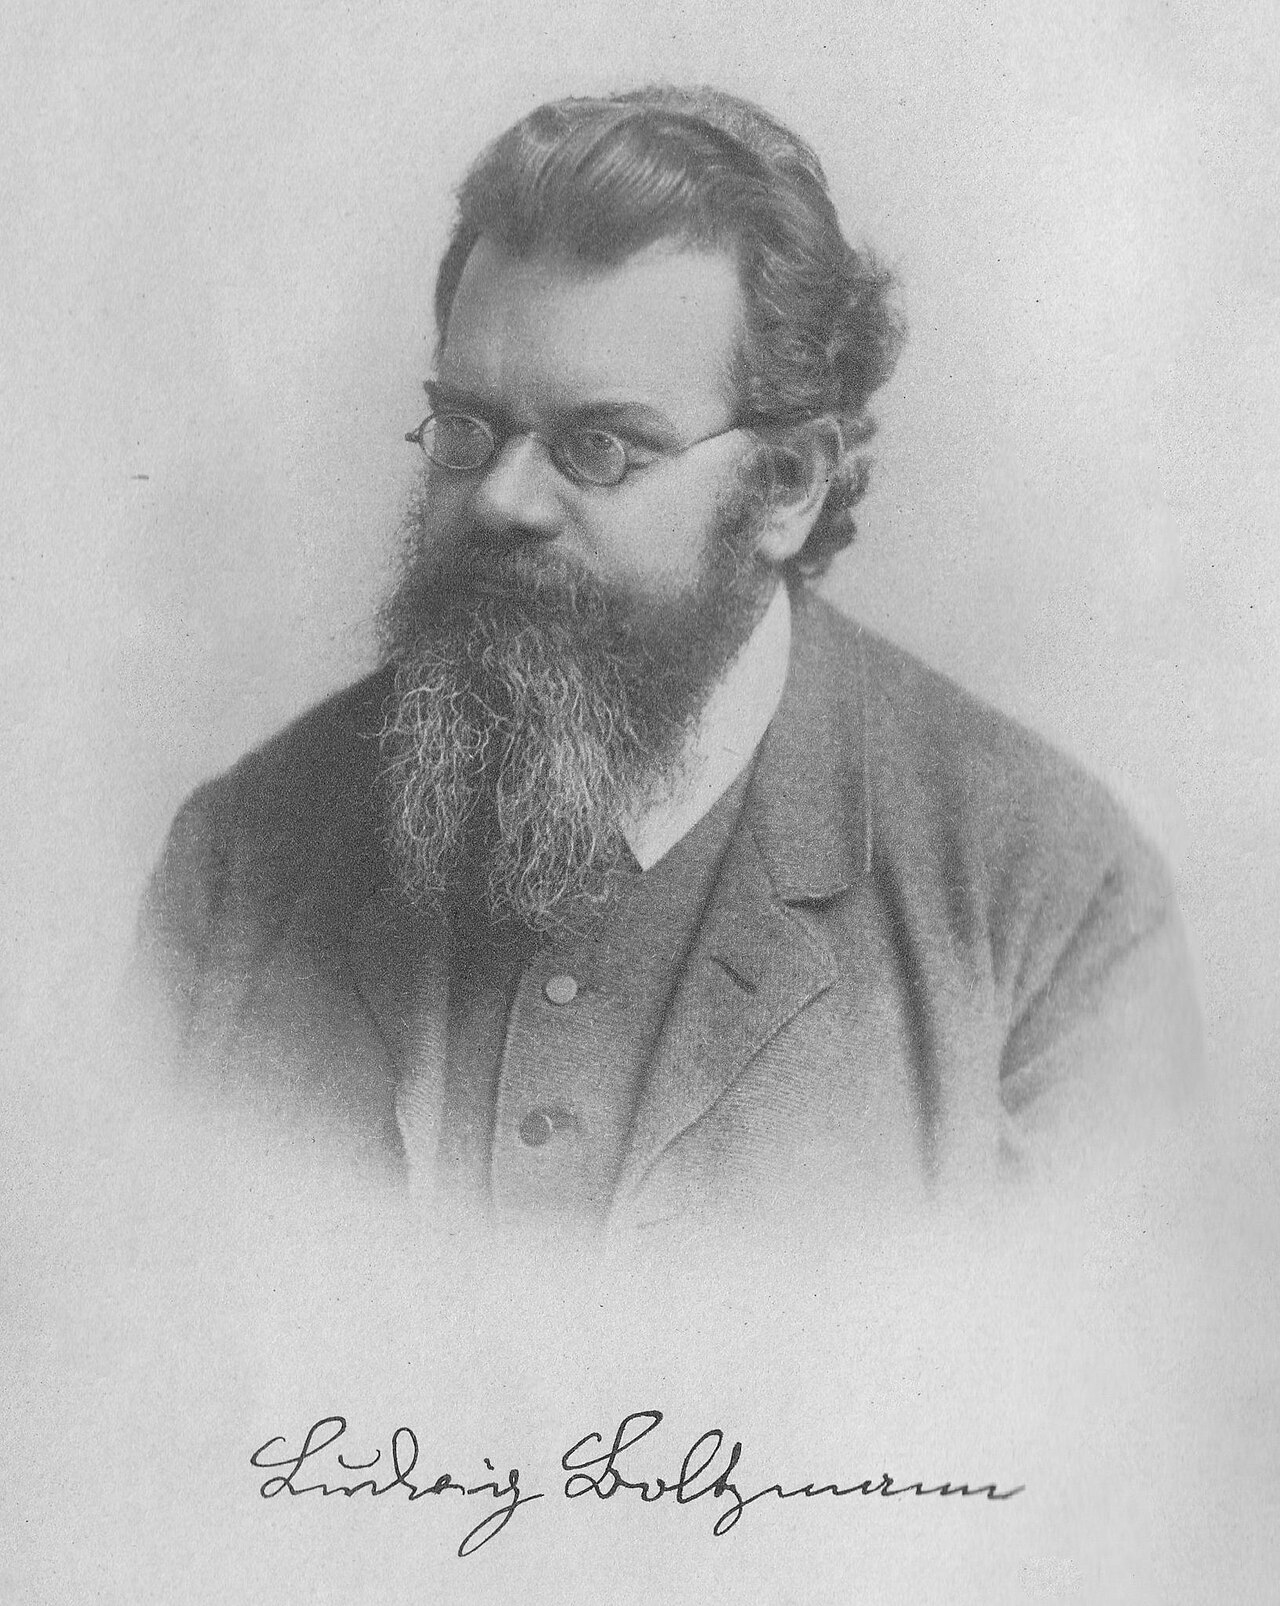
\includegraphics[width=0.3\linewidth]{images/book4/boltzmann-portrait.jpg}

{\small लुडविग बोल्ट्ज़मान (1844--1906), जिनका गुणक $\eu^{-E/k_BT}$ इस अध्याय का विषय है, और जिनका सूत्र $S = k_B\ln\Omega$ वियना में उनकी समाधि पर उत्कीर्ण है।}
\end{omfigure}

\section{समस्या: समतापी वायुमंडल, हीलियम पलायन और कोई प्रचक्रण तापमापी}

\begin{problem}[{सप्ताहांत समस्या --- एक ही चरघातांकी के तीन उपयोग}]\label{pb:b2:boltzmann-factor:1}
आँकड़े: $k_B = \qty{1.38e-23}{J/K}$, $N_A = \qty{6.02e23}{mol^{-1}}$, $g =
\qty{9.8}{m/s^2}$, $R_{\oplus} = \qty{6.37e6}{m}$, $\mu_B = \qty{9.27e-24}{J/T}$;
हवा $M = \qty{29}{g/mol}$, हीलियम \qty{4}{g/mol}, नाइट्रोजन \qty{28}{g/mol}।

\textbf{भाग I --- समतापी वायुमंडल।}
\begin{enumerate}
  \item द्रवस्थैतिकी और परिपूर्ण-गैस नियम से, $P(z) =
        P_0\eu^{-z/H}$ व्युत्पन्न कीजिए और \qty{288}{K} पर हवा के लिए $H$ दीजिए।
  \item परिणाम में बोल्ट्ज़मान गुणक पहचानिए; कौन-सी ऊर्जा,
        कौन-सा ताप?
  \item \qty{3000}{m}, \qty{5500}{m} और \qty{8849}{m} पर दाब; और वह
        ऊँचाई जहाँ दाब आधा हो जाए।
  \item प्रति वर्ग मीटर वायुमंडल का द्रव्यमान ($P_0 =
        \qty{1.013e5}{Pa}$ से), और कुल द्रव्यमान; जाँचिए कि $\int_0^\infty
        \rho\,\dd z = \rho_0H$।
  \item वायुमंडल में अणुओं की संख्या।
  \item यदि हर गैस अपना ही $H$ मानती, तो ज़मीन की तुलना में
        \qty{50}{km} पर अनुपात O$_2$/N$_2$ क्या होता? असल में
        संघटन \qty{100}{km} तक एकसमान क्यों है?
  \item असली क्षोभमंडल \qty{6.5}{K/km} पर ठंडा होता है: \qty{10}{km} पर
        दाब समतापी आकलन से ऊँचा है या नीचा?
        समझाइए।
  \item समुद्र-तल पर और \qty{100}{km} पर संख्या-घनत्व (समतापी
        मॉडल, \qty{288}{K}): ``अंतरिक्ष की देहरी'' पर टिप्पणी कीजिए।
\end{enumerate}

\textbf{भाग II --- हीलियम पलायन।}
बहिर्मंडल, \qty{500}{km} के ऊपर, लगभग \qty{1000}{K} पर और
टक्कर-रहित है: पलायन चाल से तेज़ ऊपर की ओर चलता कोई अणु
निकल जाता है।
\begin{enumerate}[resume]
  \item उस ऊँचाई पर पृथ्वी से पलायन चाल।
  \item \qty{1000}{K} पर हीलियम और नाइट्रोजन की सर्वाधिक संभाव्य तथा माध्य
        चालें।
  \item $v > v_{\text{पल}}$ वाले हीलियम परमाणुओं का अंश
        ($(2/\sqrt\pi)x\eu^{-x^2}$ लीजिए); नाइट्रोजन के लिए वही।
  \item पलायन करते हीलियम का फ्लक्स मोटे तौर पर $\tfrac14n_{\text{He}}\langle
        v\rangle \times$ (वह अंश) $\times\tfrac12$ है; बहिर्मंडल-तल पर $n_{\text{He}}
        = \qty{1e12}{m^{-3}}$ के साथ, प्रति वर्ग मीटर प्रति सेकंड और पूरी पृथ्वी के
        लिए प्रति वर्ष हानि आँकिए।
  \item हवा में हीलियम आयतन से \qty{5}{ppm} है: वायुमंडल में कुल
        हीलियम; और निकाली गई हानि के सामने उसका निवास-काल।
  \item भूपर्पटी में रेडियोऐक्टिवता प्रति वर्ष लगभग \qty{3e6}{kg} हीलियम
        बनाती है: क्या वायुमंडल का हीलियम स्थायी अवस्था में है, और
        प्रश्न 11 से तुलना क्या सिखाती है?
  \item सौर उच्चतम पर बहिर्मंडल \qty{2000}{K} तक पहुँचता है: हीलियम
        पलायन अंश किस गुणक से चढ़ता है?
  \item चंद्रमा के पास कोई वायुमंडल क्यों नहीं, और टाइटन (पलायन
        \qty{2.6}{km/s}, \qty{94}{K}) के पास मोटा क्यों?
\end{enumerate}

\textbf{भाग III --- कोई प्रचक्रण तापमापी।}
किसी अनुचुंबकीय लवण में $n = \qty{2e27}{m^{-3}}$ प्रचक्रण 1/2 हैं जिनका $\mu
= \mu_B$ है, किसी क्षेत्र $B$ में।
\begin{enumerate}[resume]
  \item दोनों स्तरों की जनसंख्याएँ और चुंबकन
        $M(B,T)$।
  \item $B = \qty{0.1}{T}$ पर: \qty{300}{K}, \qty{4}{K}, \qty{0.05}{K} पर $M$;
        \omterm{prop:b2:boltzmann-factor:curie}{क्यूरी का नियम} कहाँ मान्य है?
  \item $M$ कोई तापमापी क्यों है, और किस परास में वह सबसे
        संवेदी है? व्यवहार में क्या मापा जाता है?
  \item प्रचक्रणों की माध्य ऊर्जा और ऊष्मा-धारिता (शॉट्की);
        \qty{0.1}{T} पर शिखर का ताप।
  \item ऊँचे और शून्य ताप पर प्रचक्रणों की एंट्रॉपी; $T \to 0$ होते
        कौन-सा ``क्रमण'' होता है?
  \item \qty{1}{K}, \qty{1}{T} से \qty{0.01}{T} तक रुद्धोष्म विचुंबकन:
        अंतिम ताप; $B \to 0$ से $T \to 0$ क्यों नहीं मिल सकता?
  \item कोई नाभिकीय-प्रचक्रण तापमापी $\mu_{\text{N}} = \mu_B/1836$ लेता है:
        \qty{1}{T} पर, किस ताप तक \omterm{prop:b2:boltzmann-factor:curie}{क्यूरी का नियम} टिकता है, और
        ऐसा तापमापी माइक्रोकेल्विन परास में क्यों काम आता है?
  \item किसी वर्णक्रमी रेखा की डॉप्लर चौड़ाई (मैक्सवेल के
        वितरण से) की गैसों के तापमापी के रूप में तुलना कीजिए: कौन-सी राशि, और
        वह $T$ के साथ कैसे मापती है?
  \item सारांश दीजिए: तीन निकाय और वह एक ही सूत्र।
\end{enumerate}
\end{problem}
